\documentclass[11pt,twocolumn,a4paper]{article}
\usepackage[utf8]{inputenc}
\usepackage[english,german]{babel}
\usepackage{utopia}
\usepackage[left=.3in,right=0.3in,top=.8in,bottom=.8in]{geometry}
\usepackage[parfill]{parskip}
\usepackage{makeidx}
\usepackage[onehalfspacing]{setspace}
\usepackage{fancyhdr}
\usepackage{lastpage}
\usepackage{hyperref}
\usepackage{amssymb}
\usepackage{graphicx}
\newcommand*{\field}[1]{\mathbb{#1}}%
\renewcommand{\sffamily}{phv}

\newcommand{\titleText}{Spick Mathematik 14. November 2016}
\newcommand{\authorText}{Patrick Günthard}
\newcommand{\dateText}{\today}

\title{\titleText}
\author{\authorText}
\date{\dateText}

\pagestyle{fancy}
\fancyhf{}

\fancyhead[L]{\titleText}
\fancyhead[R]{\authorText}
\cfoot{\thepage \space von \pageref{LastPage}}

\begin{document}
\section{Potenzfunktionen}
\textbf{Grundform:}\\
\(f(x) = x^n\)\\Wobei \(n \in \field{N}\)\\
\textbf{Graph:}\\
\frame{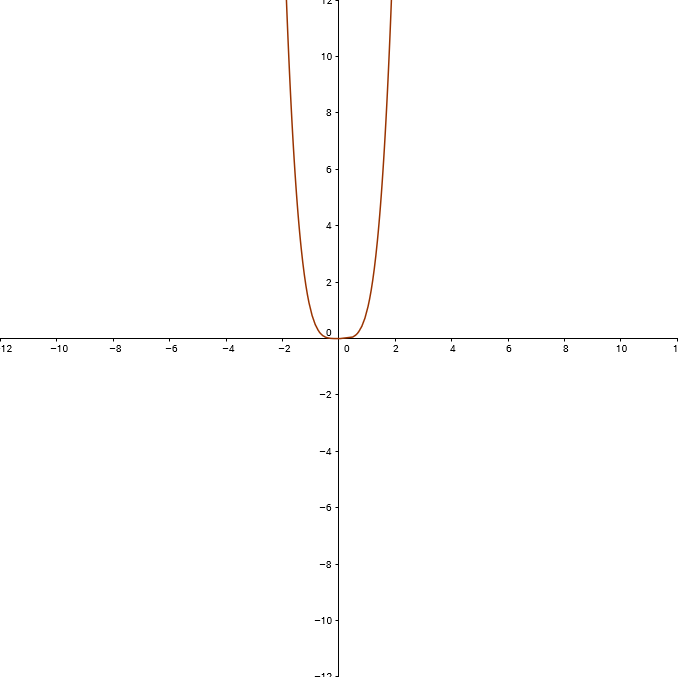
\includegraphics[width=4cm]{graphs/potenz1}}\(f(x) = x^{2n}\)\\
\frame{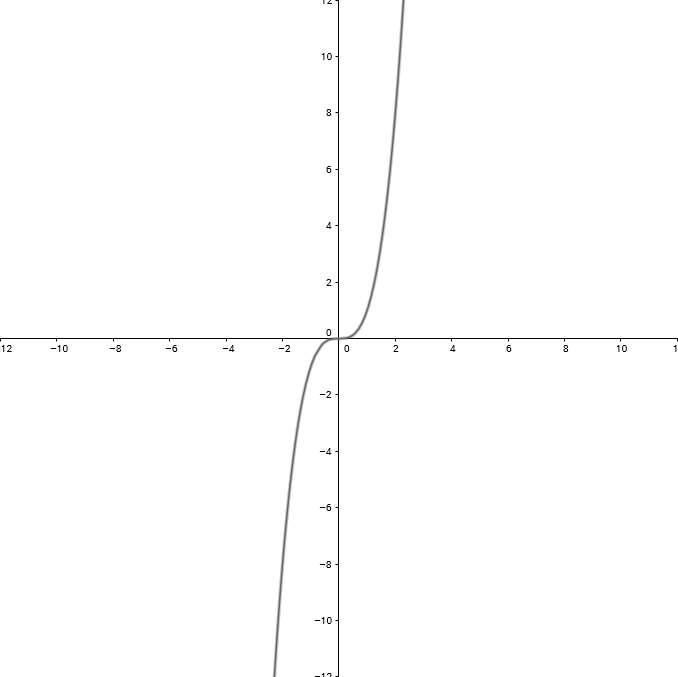
\includegraphics[width=4cm]{graphs/potenz2}}\(f(x) = x^{2n-1}\)
\section{Polynomfunktion}
\textbf{Grundform:}\\
\(f(x) = a_nx^n + a_{n-1}x^{n-1} + \dots + a_2x^2 + a_1x + a \)\\
Wobei: \(n \in \field{N}\) und \(a_i \in \field{R}\) und \(a_n \ne 0\)\\
\textbf{Annäherungen:} (Bsp: \(f(x)=8x^4+x^3-2x^2+6\))\\
Für kleine \(|x|\) Werte: \(f(x) \approx -2x^2 + 6\)\\
Für grosse \(|x|\) Werte: \(f(x) \approx 8x^4\)
\textbf{Graph:}\\
\frame{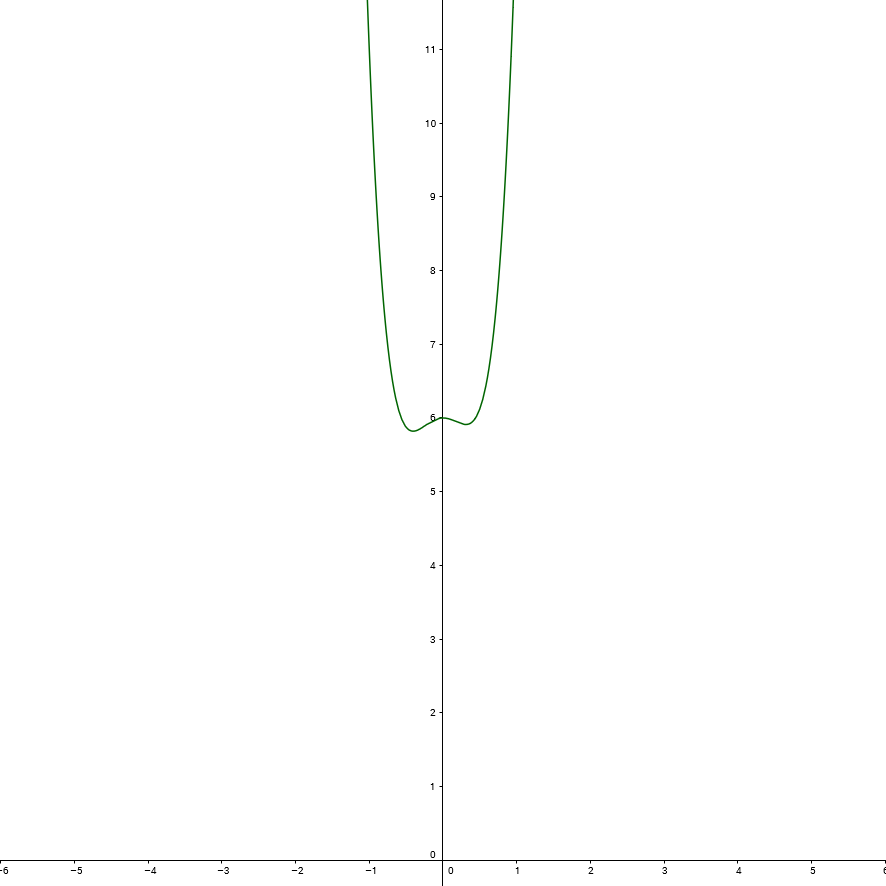
\includegraphics[width=4cm]{graphs/polynom}}
\section{Rationale Funktionen}
\textbf{Grundform:}\\ \(f(x) =
\frac{Z(x)}{N(x)}\)\\ \textbf{Polstelle:}\\ Argument \(x=a\) wo \(N(a)
= 0\) und \(Z(a) \ne 0\)\\ \textbf{Asymptote:}\\ Nähert sich eine Kurve immer
mehr einer Geraden, ohne sie zu schneiden oder zu berühren, so heisst diese
Gerade \textit{Asymptote}.\\
\textbf{Graph:}\\
\frame{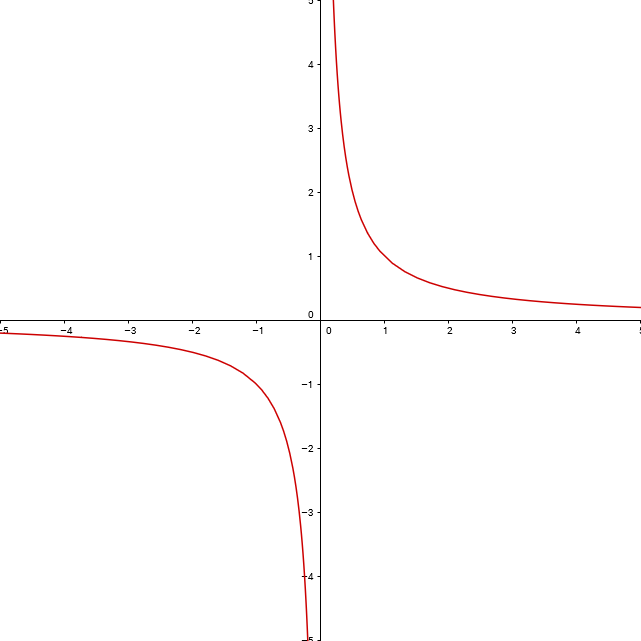
\includegraphics[width=4cm]{graphs/rational1}}
\frame{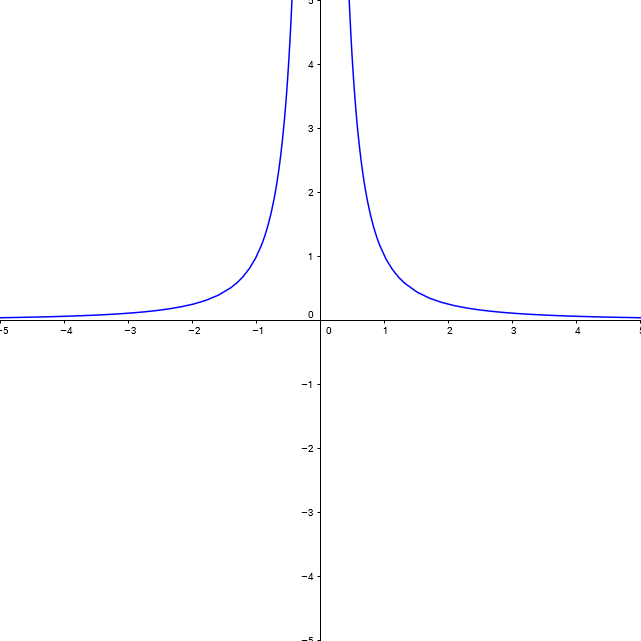
\includegraphics[width=4cm]{graphs/rational2}}
\end{document}
